\section{Approcci scartati}

\subsection{Modello ad Agente su spazio continuo}
L'idea alla base era qualla di modellare una popolazione tramite l'utilizzo di 
uno spazio del modello di tipo continuo. Gli agenti sarebbero poi stati modellati come 
individui singoli e reali, in quanto entita' effettivamente attive all'interno 
dello spazio. Ci si puo' immaginare lo spazio del modello come una grande griglia 
definita da coordinate \emph{continue} di una certa dimensione \emph{$N \times M$}. All'interno 
di questa griglia vengono posizionati randomicamente gli agenti, i quali vengono 
rappresentati graficamente come dei punti di differenti colori.

\begin{minipage}{\linewidth}
    \centering
    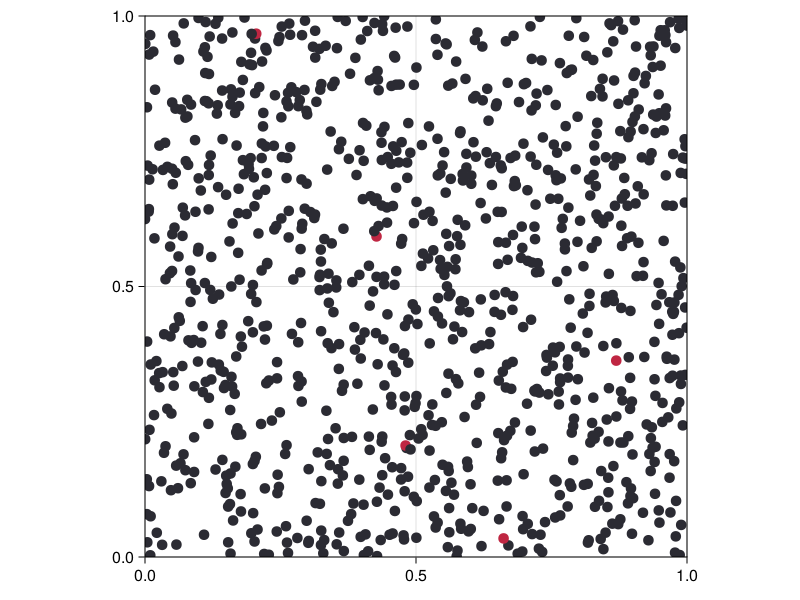
\includegraphics[width=\textwidth]{img/ball-covid.png}
    \captionof{figure}{Esempio del modello modellato su spazio continuo}
    \label{fig:ball_covid}
\end{minipage}

Questo approccio utilizzava una metodologia similare a quella delle palline da biliardo 
per modellare l'interazio tra agenti all'interno dello spazio del modello. Ogni agente poteva
infettare in maniera casuale un suo vicino sse i due avevano un interazione. Ogni interazione
era modellata similmente ad un urto elastico \cite{wiki:Urto_elastico} tra corpi. 
Questo non era tuttavia un simulatore di urti elastici affidabili, bensi' un approccio che prendeva
spunto da esso, in particolare dal gioco del biliardo. 

In questo modo il comportamento complessivo del modello poteva permettere l'osservarsi 
di un andamento simile a quanto ci si aspetterebbe da un sistema simile.

\begin{minipage}{\linewidth}
    \centering
    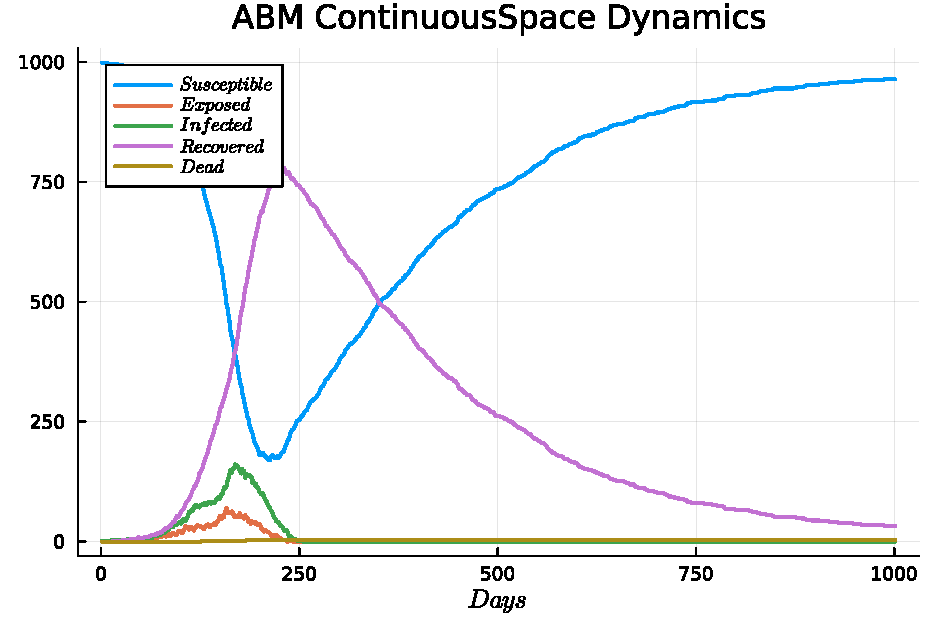
\includegraphics[width=\textwidth]{img/plot_abm_continuousspace.pdf}
    \captionof{figure}{Esempio del comportamento delle curve nel modello continuo}
    \label{fig:seir_curve_continuous}
\end{minipage}

Sono state poi implementate svariate proprieta' come la proprieta' di essere individuati 
dopo un periodo di latenza come individui infetti e quindi essere confinati in quarantena, 
la quale era definita come una diminuzione nella probabilita' di infettare ed essere infettati 
perdendo la capacita' di muoversi.

Questa tipologia di approccio, quella Agent oriented, richiedeva una quantita' di risorse computazionali 
e di tempo estremamente elevato in relazione al numero di agenti presenti nel modello. Questo approccio 
inoltre e' stato valutato come troppo granulare e inadatto allo scopo del progetto. 
Si e' deciso quindi di adottare un approccio meno granulare e piu' flessibile 
andando ad un livello di astrazione piu' alto.

\subsection{Modello ad Agente con spazio a grafo e modellazione singolo agente}
L'idea e' nata per cercare di avere un controllo piu' granulare sullo spazio del modello e sulla sua 
evoluzione locale, non tanto degli agenti. Sono nati molteplici problemi, primo tra tutti quello del tempo impiegato
e successivamente quello del comportamento delle curve epidemiologiche che non rispettavano 
assolutamente il comportamento descritto dal modello deterministico SEIR, ma non in un modo 
ragionevole, bensi' in un modo completamente alieno. 

\begin{minipage}{\linewidth}
    \centering
    \includegraphics[width=\textwidth]{img/COMPARISON DIFFERENT R₀ VALUE_2023-06-29.pdf}
    \captionof{figure}{Comportamento modello ABM su spazio a grafo al variare del parametro $R_0$}
    \label{fig:strange_behaviour_R0_abm}
\end{minipage}

\begin{minipage}{\linewidth}
    \centering
    \includegraphics[width=\textwidth]{img/COMPARISON DIFFERENT R₀ VALUE_2023-06-29 (1).pdf}
    \captionof{figure}{Comportamento modello SEIR al variare del parametro $R_0$}
    \label{fig:strange_behaviour_R0_ode}
\end{minipage}

Si puo' facilmente osservare come il comportamento delle curve prenda un comportamento 
anomalo fin dalle prime variazioni del parametro $R_0$ per culminare con risultati 
completamente alieni. Il motivo alla base rimane tutt'ora ignoto e sconosciuto, tuttavia
esecuzioni differenti hanno mostrato dei comportamenti differenti, seppur altrettanto 
alieni. 

Questo comportamento pero' puo' essere descritto a grandi linee dalla seguente formula

\begin{minipage}{\linewidth}
    \centering
    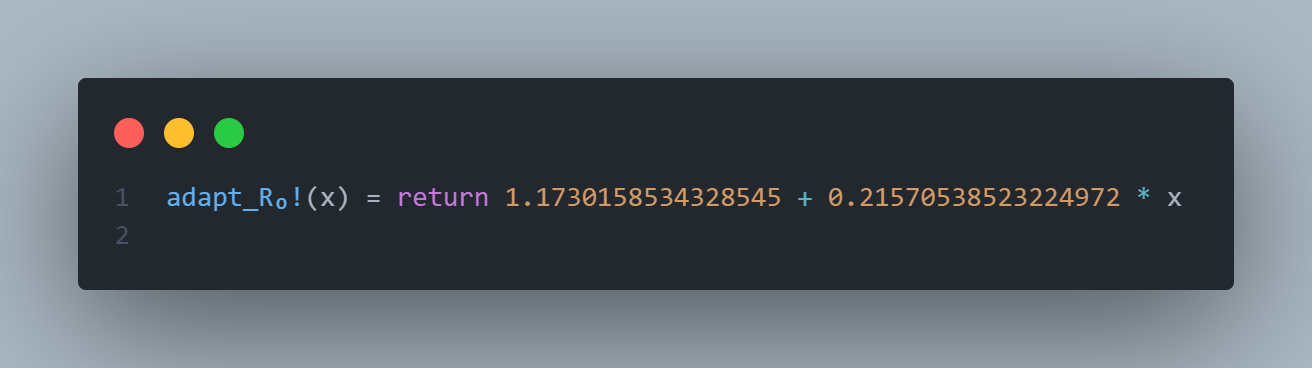
\includegraphics[width=\textwidth]{img/rapporto_strano.png}
    \captionof{figure}{Formula che si occupa di descrivere il rapporto tra il comportamento del modello scartato e del modello SEIR. In particolare questa formula descrive il rapporto tra gli $R_0$}
    \label{fig:strange_behaviour_R0}
\end{minipage}

Bisogna tuttavia precisare come run successive abbiano portato a risultati differenti dei plot 
relativi al comportamento del modello ad agente. Il motivo rimane tutt'ora ignoto ma e' possibile
che uno degli attori in gioco possa essere la funzione \textbf{random} associata al campionamento 
degli individui che va a fare da mimica per il numero di contatti che avvengono ad ogni passo 
per ogni individuo infetto. Questo campionamento si basa principalmente sul calcolo di una 
distribuzione di \textbf{Poisson} \cite{wiki:Distribuzione_di_Poisson} con parametro $\lambda = R_0$.

In particolare la formula e' stata ricavata dopo aver fatto un confronto tra molteplici 
valori di $R_0$ e i risultati ottenuti sia dal modello SEIR che dal modello ABM. 
Successivamente e' stato calcolato \textbf{MSE} (Medium Square Error) per ogni coppia possibile
di risultati per cercare quelli tra loro piu' simili, andando ad ottenere quindi un insieme
di coppie. Queste poi sono state inserite in un metodo che calcolava una \textbf{polynomial fit} \cite{wiki:Polynomial_regression}
tra tutte le coppie di valori per vedere quale poteva essere la formula che governava la differenza 
di risultati. Da tenere a mente che in un caso normale questa differenza non dovrebbe esistere, 
o quanto meno se esiste dovrebbe essere trascurabile.

\begin{figure}[!hb]
	\centering
	\begin{subfigure}[b]{0.45\textwidth}
		\centering
		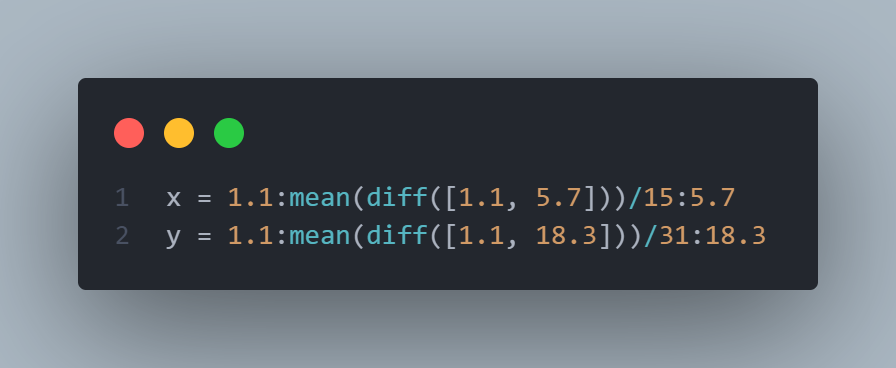
\includegraphics[width=\textwidth]{img/r0_range_test.png}
    	\caption{figure}{Range di valori di $R_0$ testati}
    	\label{fig:r0_range_test}
	\end{subfigure}
	\hfill
	\begin{subfigure}[b]{0.45\textwidth}
		\centering
		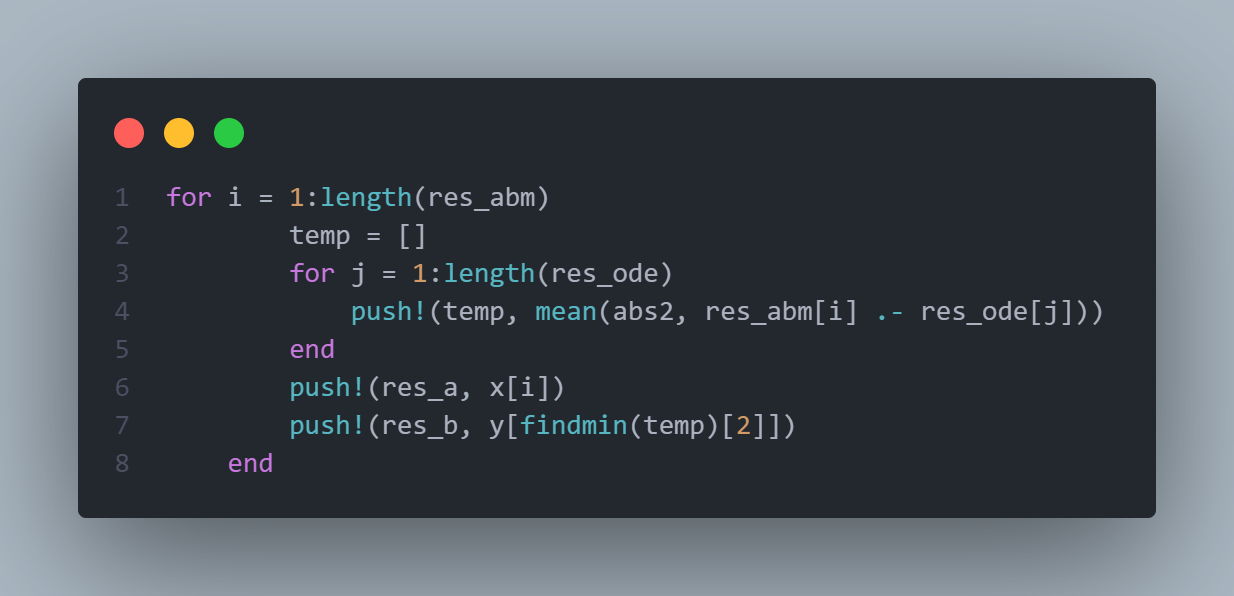
\includegraphics[width=\textwidth]{img/mse_r0.png}
		\caption{Calcolo MSE risultati SEIR - ABM}
		\label{fig:mse_r0}
	\end{subfigure}
\end{figure}

Da qui si ottiene la formula in figura \ref{fig:strange_behaviour_R0} la quale descrive approssimativamente, 
in base al grado del polinomio che si vuole andare a creare, la relazione che esiste tra le coppie 
di valori analizzate.

La motivazione per cui il modello ad agente si comporta in maniera cosi' inaspettata
rispetto a come dovrebbe non e' stato chiaro, e in letteratura non sembra esserci alcun 
articolo che ne parli in maniera approfondita, e per questo ho deciso di abbandonare l'approccio.
Punto a favore e' stato anche il fatto che l'approccio con ABM era estremaente esoso in termini 
di risorse computazionali e tempistiche. Questo problema e' insito in ogni tipo di simulazione, 
tuttavia affiancato allo stravagante problema comparso e descritto sopra, e' stato 
decisivo per il cambio drastico di approccio. 

\subsection{Controllore Ipopt}
Ipopt (Interior Point OPTimizer) \cite{Wächter2006} e' un pacchetto software per 
l'ottimizzazione non lineare su larga scala. Questo pacchetto software e' realizzato 
per trovare delle soluzioni (locali) a problemi di ottimizzazione matematica nella forma:
$\min_{x \in R^n} f(x)$ tale che $g_L \leq g(x) \leq g_U$ e $x_L \leq x \leq x_U$, dove 
$f(x): R^n \rightarrow R$ e' la funzione obiettivo e $g(x): R^n \rightarrow R^m$ 
sono le funzioni di vincolo.

I vettori $g_L$ e $g_U$ denotano i limiti inferiore e superiore sui vincoli e i vettori
$x_L$ e $x_U$ sono i limiti delle variabili $x$. Le funzioni $f(x)$ e $g(x)$ possono essere 
sia non lineari che non convesse, ma la loro derivata seconda deve esistere e deve essere 
continua.

\begin{minipage}{\linewidth}
    \centering
    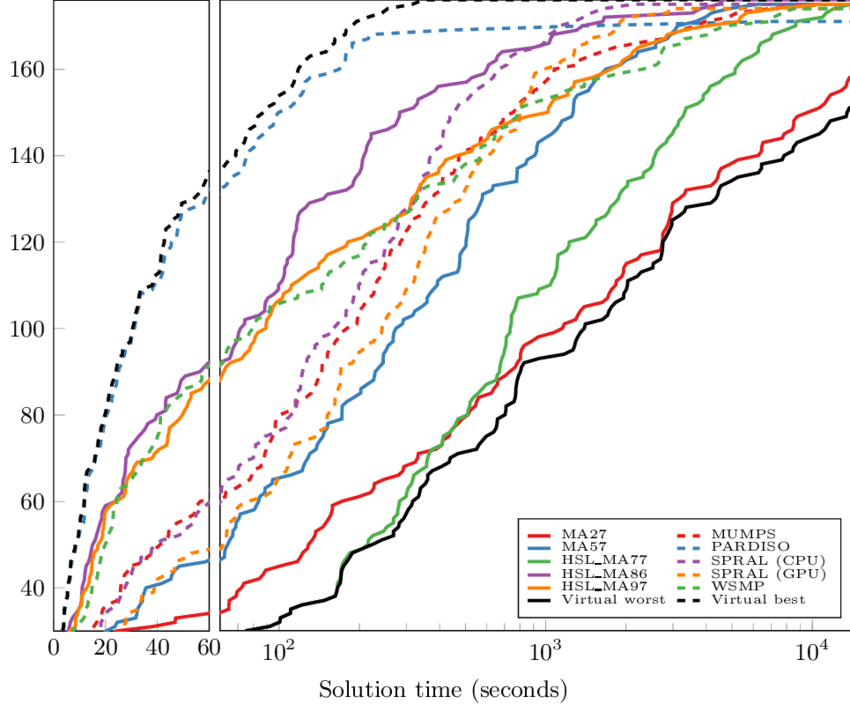
\includegraphics[width=\textwidth]{img/Comparison-of-Ipopt-performance-over-various-linear-solvers-using-the-two-dimensional.png}
    \captionof{figure}{Comparison of Ipopt performance over various linear solvers using the two-dimensional partial differential equation test problem set. \cite{unknown}}
    \label{fig:Ipopt_solver}
\end{minipage}

Ipopt e' scritto in \textbf{C++} ed e' stato rilasciato come software open source sotto la licenza \textbf{Eclipse Public License (EPL)}.

L'utilizzo della suite \textbf{Ipopt} e' stato fatto per l'applicazione di un sistema
di monitoraggio e intervento all'interno del modello di simulazione. Successivamente l'idea
di utilizzare un integrazione con la suite \textbf{SciML.ai} verra' sfruttata per 
aggiungere algoritmi di Machine Learning per rendere piu' realistico e consistente il modello 
nelle sue predizioni e scelte.

\begin{minipage}{\linewidth}
	\centering
	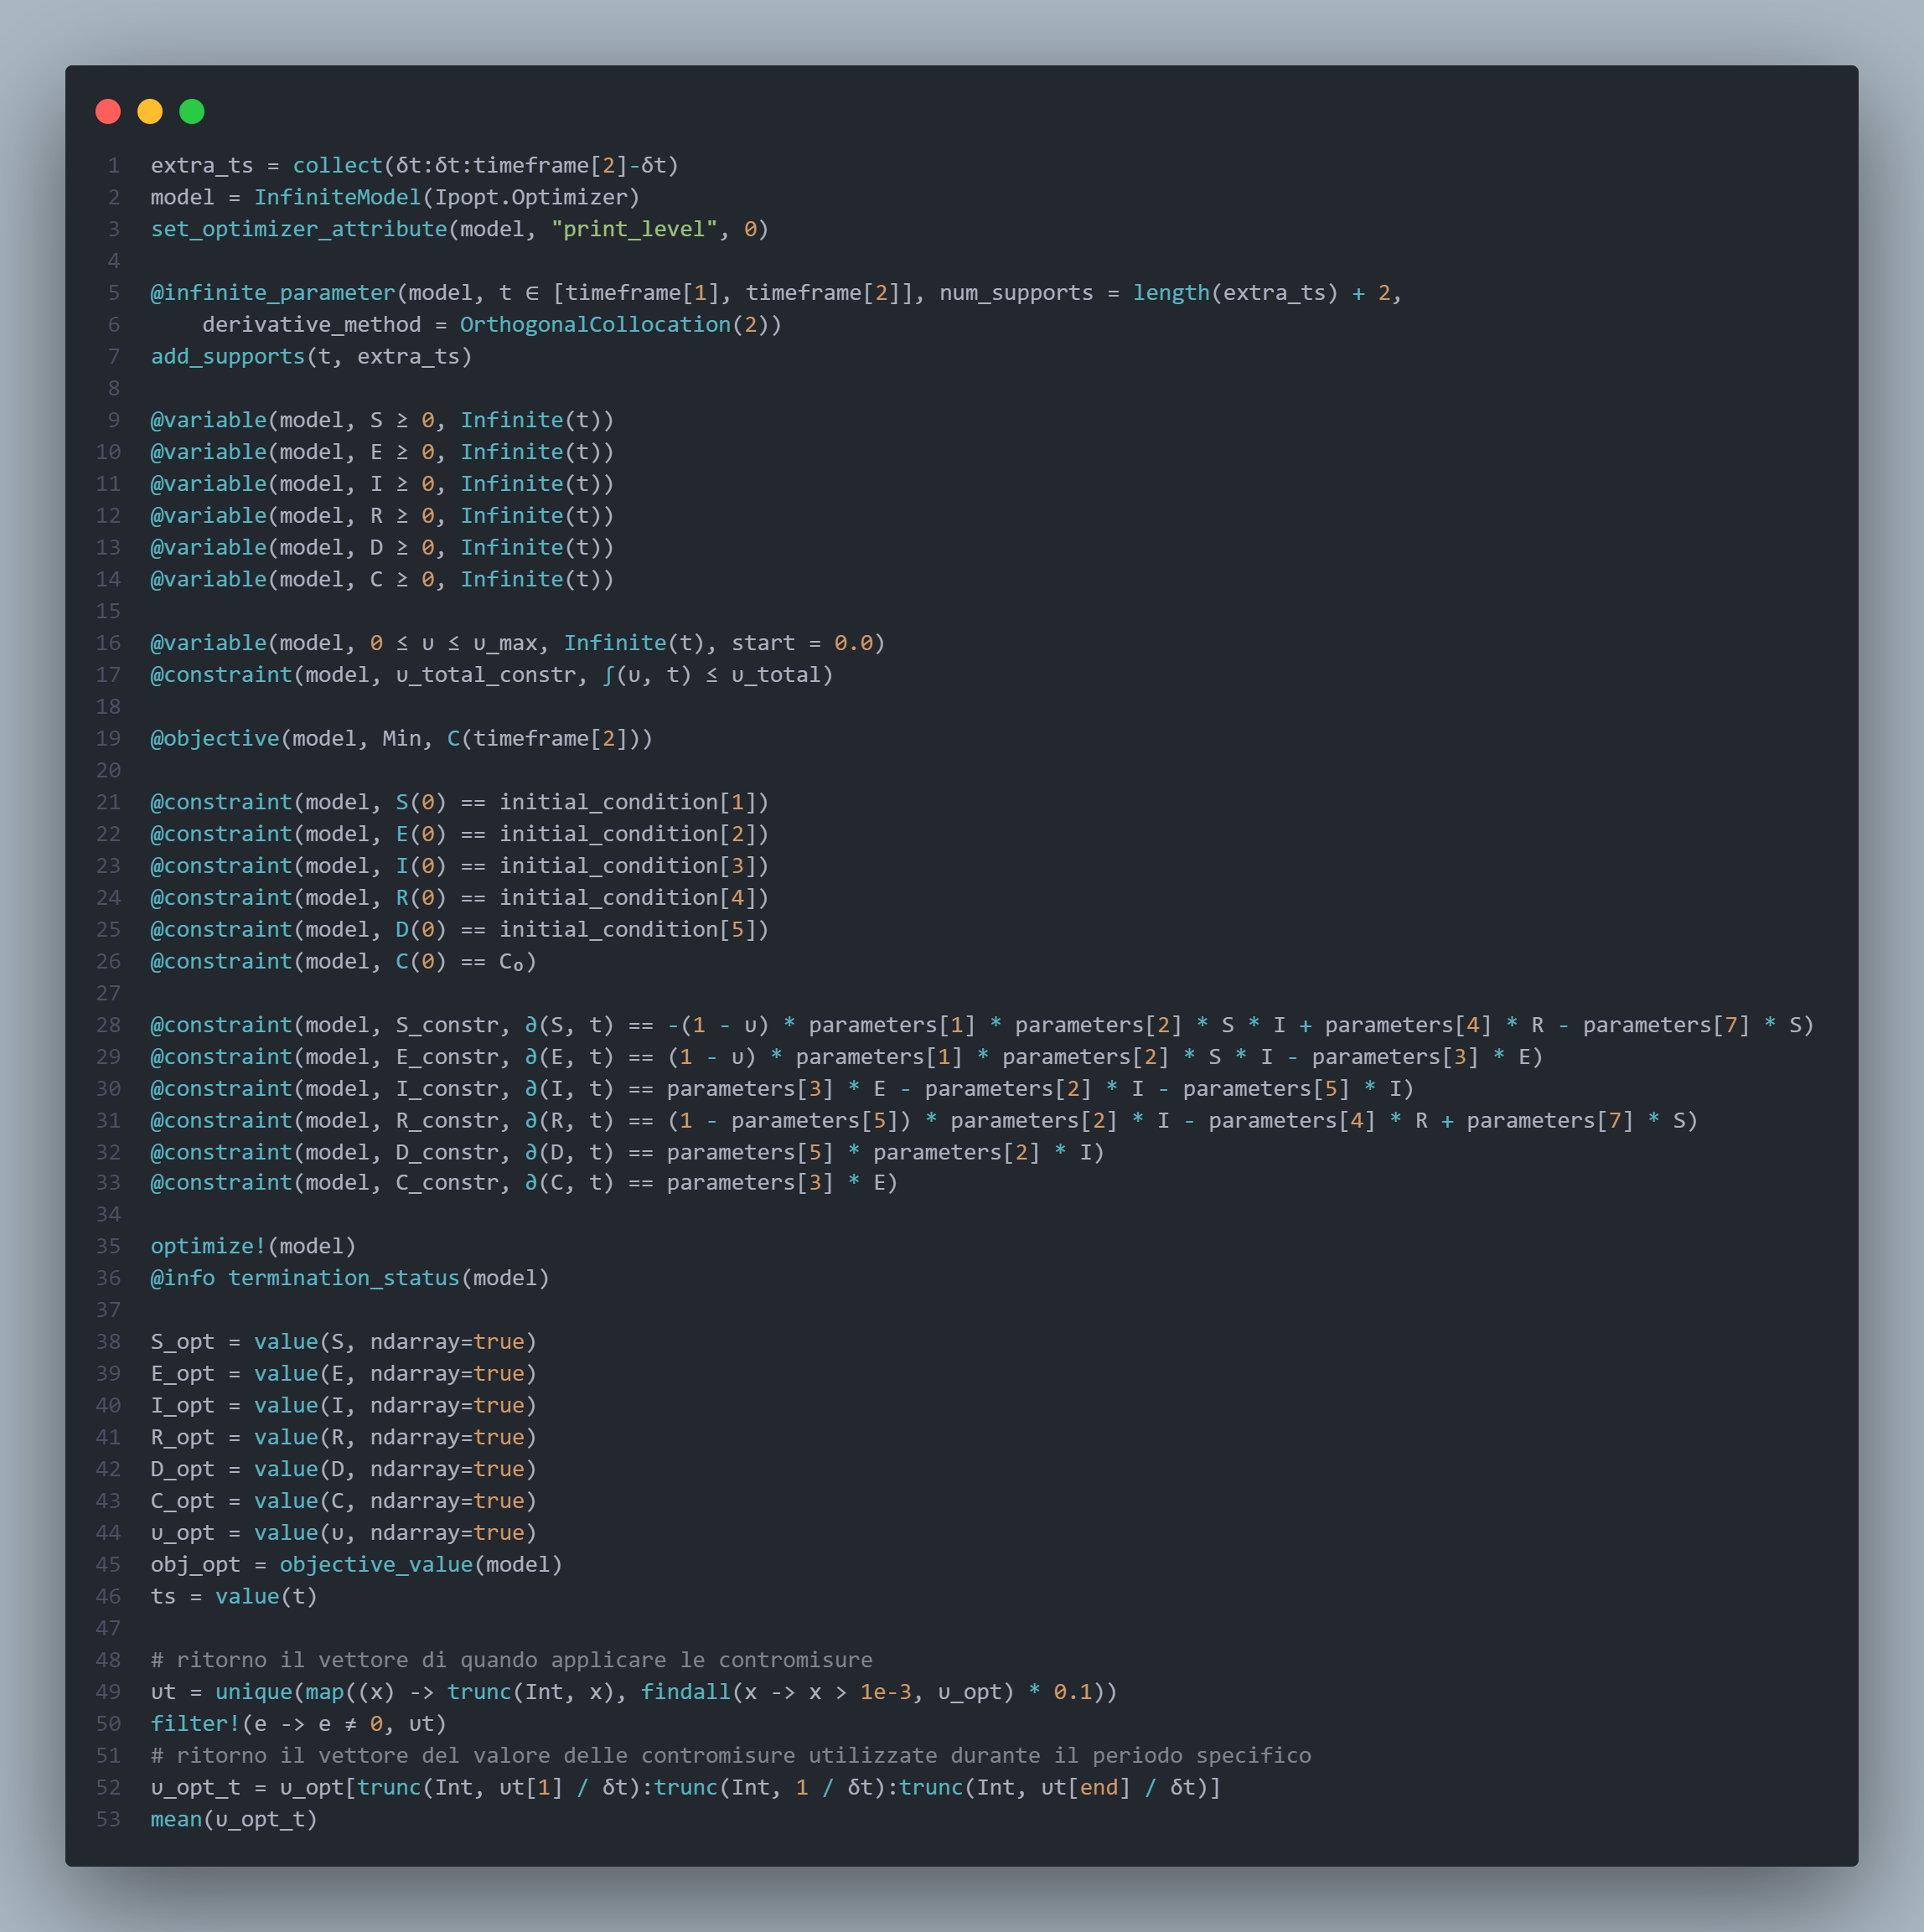
\includegraphics[width=\textwidth]{img/controller_ipopt.png}
	\captionof{figure}{Definizione del controllore tramite Ipopt}
	\label{fig:controller_ipopt}
\end{minipage}

L'approccio generale e' stato semplice ma efficace, in quanto viene definito un modello 
per raccogliere tutte le informazioni relative e necessarie per l'algoritmo di ottimizzazione
e successivamente vengono definite le regole che governano il comportamento del modello. 

Le regole in questione sono principalmente le stesse che sono usate per descrivere il modello SEIR
che viene utilizzato all'interno del modello ad agente.

\begin{minipage}{\linewidth}
	\centering
	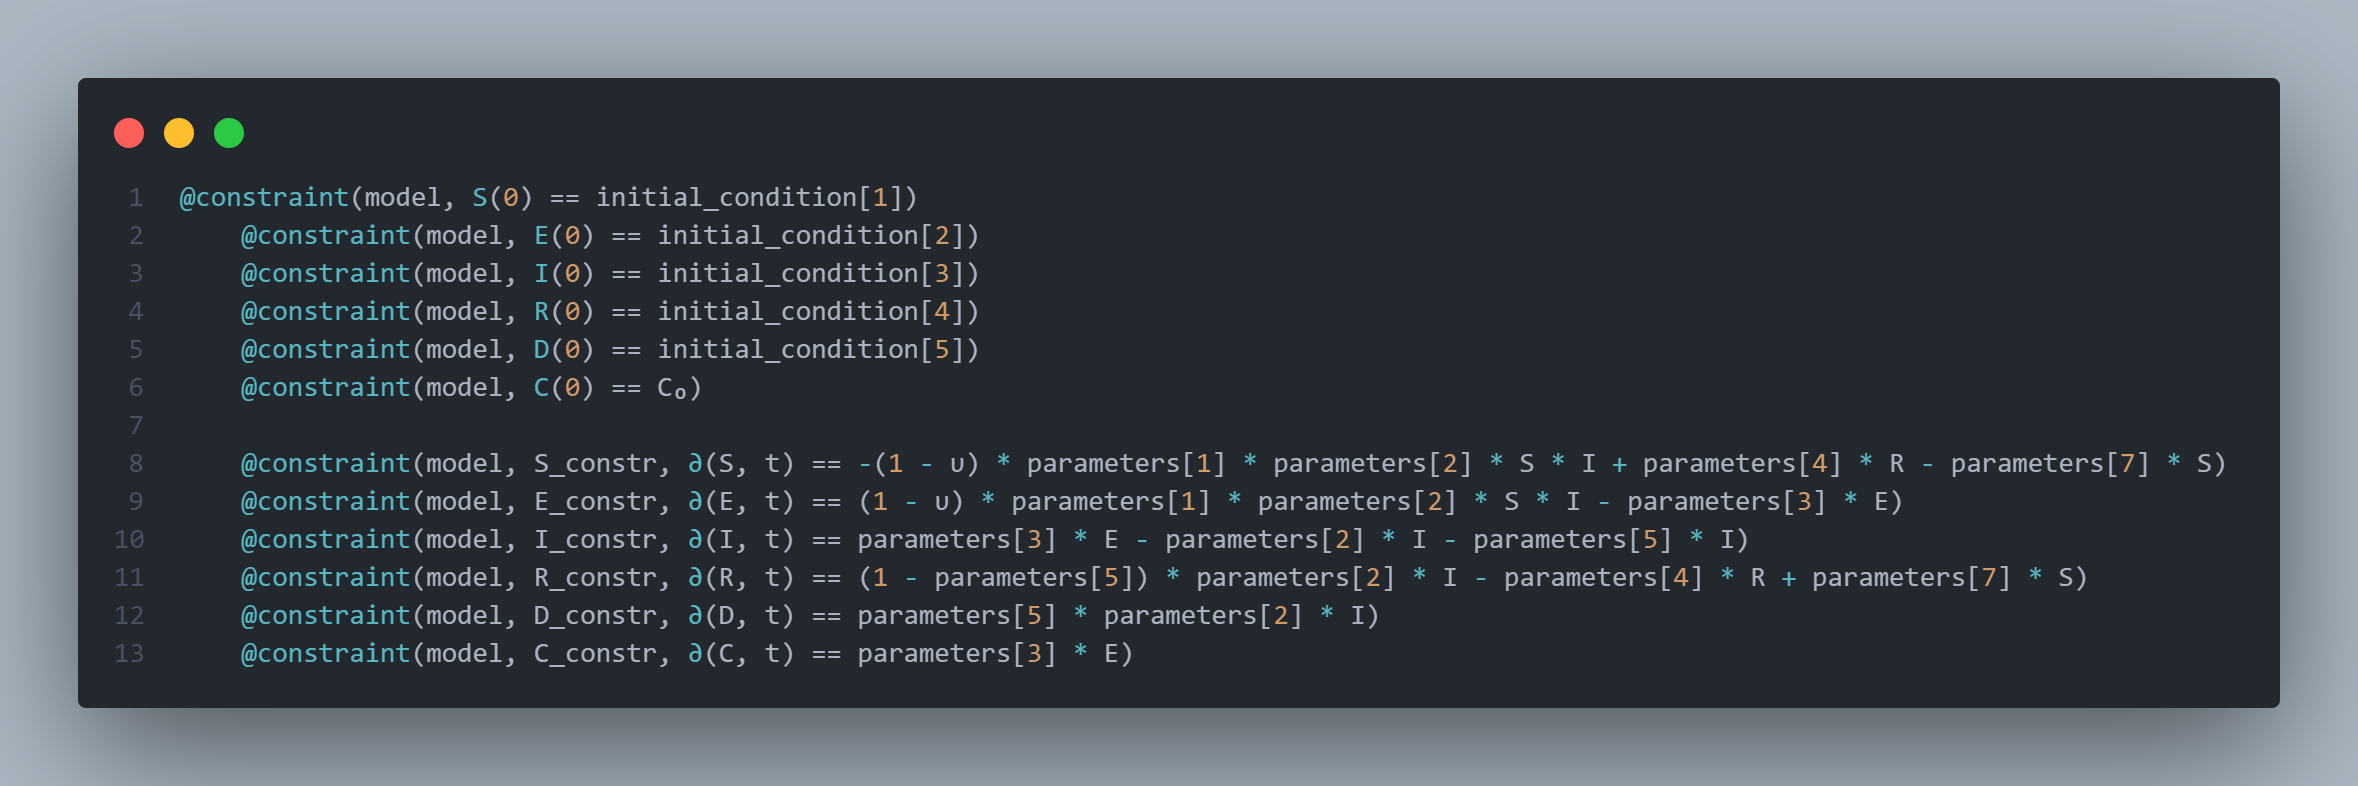
\includegraphics[width=\textwidth]{img/controller_rules.png}
	\captionof{figure}{Definizione regole del modello del controller}
	\label{fig:controller_rules}
\end{minipage}

Essendo che le regole mostrate in figura \ref{fig:controller_rules} sono relative agli stati 
SEIR e l'idea alla base del controllore e' quella di ridurre quanto piu' possibile il numero di
infetti cumulati che ci sono all'interno del sistema, e' stato aggiunto uno stato che descrive
appunto questo stato aggiuntivo.

Successivamente vi sono delle regole su quanto il modello puo' impiegare in termini di risorse, 
le quali sono le nostre contromisure con relativo costo, dato dall'integrale del valore della nostra
contromisura applicata nel tempo. Infine viene ottimizzato il modello e ritornato il valore medio delle contromisure applicate
quando applicate. 

\begin{minipage}{\linewidth}
	\centering
	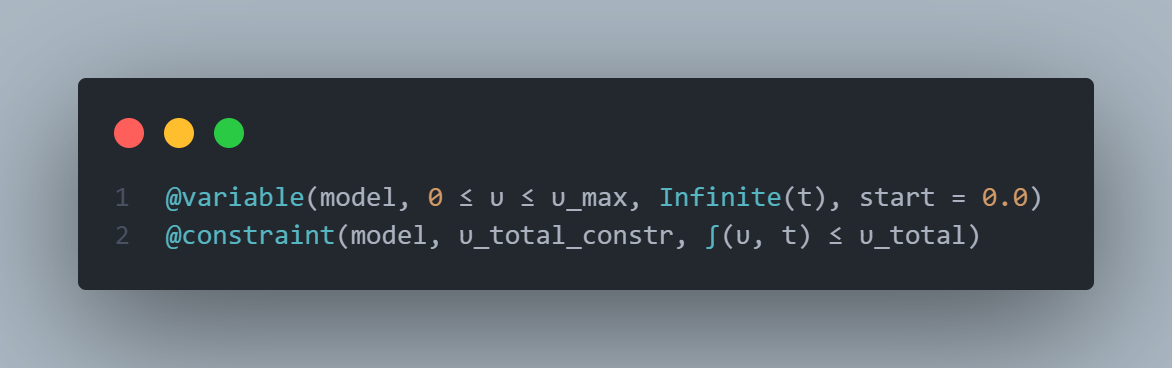
\includegraphics[width=\textwidth]{img/controller_rules_1.png}
	\captionof{figure}{Definizione regole del modello del controller per le contromisure}
	\label{fig:controller_rules_1}
\end{minipage}

I risultati ottenuti \ref{fig:ipopt_res1} \ref{fig:ipopt_res2} non si discostano troppo da quelli ottenuti tramite l'utilizzo del controllore con 
NeuralODE \ref{fig:controller1} implementato come mostra la figura \ref{fig:abm_intervent} \ref{fig:abm_all}. Si puo' notare
come i risultati siano molto simili, e per questo e' stato deciso di mantenere l'utilizzo dell'implementazione 
custom su quella della librearia Ipopt, in quanto questa scelta sembrava portare un aumento prestazionale non 
troppo significativo, ma sicuramente incoraggiante.

\begin{figure}[!hb]
	\centering
	\begin{subfigure}[b]{\textwidth}
		\centering
		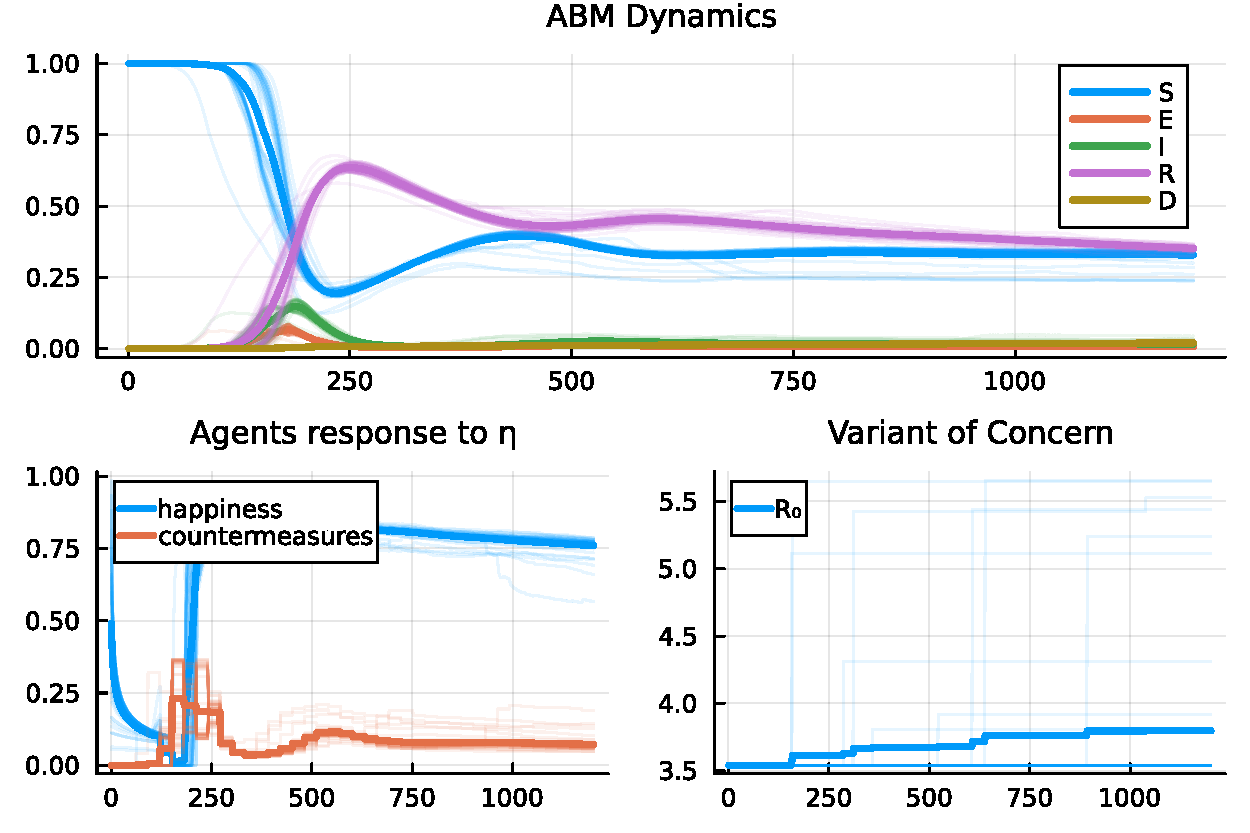
\includegraphics[width=\textwidth]{img/SocialNetworkABM_IPOPT_CONTROL.pdf}
		\caption{Risultato applicazione controllore tramite la suite Ipopt}
		\label{fig:ipopt_res1}
	\end{subfigure}
	\hfill
	\begin{subfigure}[b]{\textwidth}
		\centering
		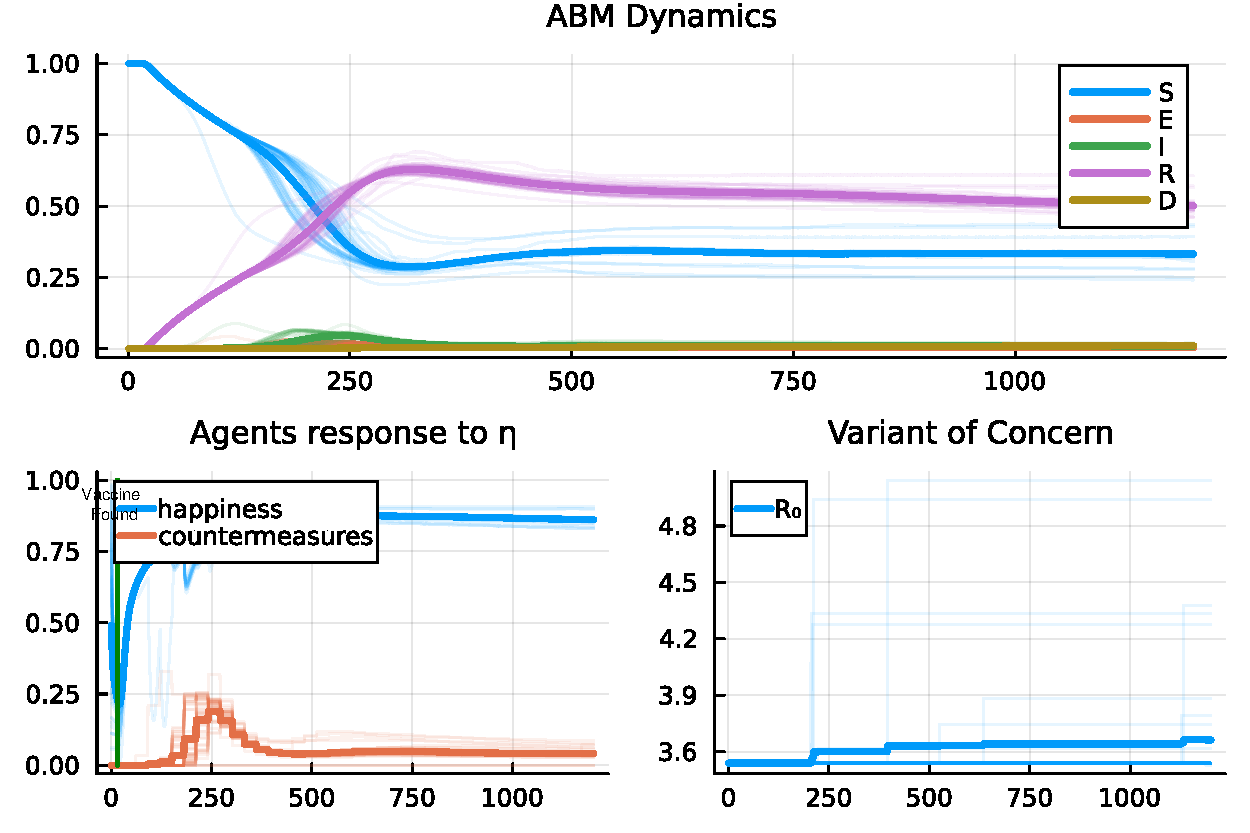
\includegraphics[width=\textwidth]{img/SocialNetworkABM_IPOPT_ALL.pdf}
		\caption{Risultato applicazione controllore tramite la suite Ipopt}
		\label{fig:ipopt_res2}
	\end{subfigure}
\end{figure}

Da notare come la possibilita' di convertire il codice da \textbf{CPU based} a \textbf{GPU based} tramite
l'ausilio di poche semplici istruzioni, sia qualcosa che e' stato preponderante nella scelta di non 
utilizzare la libreria esterna Ipopt, soprattutto in vista di possibili sviluppi futuri legati al miglioramento 
delle performance del codice in termini di risorse computazionali e soprattutto temporali.

La scelta di utilizzare un approccio ibrido come controllore piuttosto che un approccio definito tramite una suite
di ottimizzazione non lineare, e' stato optato anche in vista del fatto che la definizione del controllore diveniva 
piu' semplice rispetto alla controparte Ipopt. Questa semplicita' tuttavia e' data dal fatto che non si ha diretto 
controllo sulla funzione da ottimizzare in quanto e' mascherata da una rete neurale, cosa che con il controllore 
esplicito di Ipopt era possibile fare definendo vari vincoli sul sistema in questione.
